% (The MIT License)
%
% Copyright (c) 2023-2024 Yegor Bugayenko
%
% Permission is hereby granted, free of charge, to any person obtaining a copy
% of this software and associated documentation files (the 'Software'), to deal
% in the Software without restriction, including without limitation the rights
% to use, copy, modify, merge, publish, distribute, sublicense, and/or sell
% copies of the Software, and to permit persons to whom the Software is
% furnished to do so, subject to the following conditions:
%
% The above copyright notice and this permission notice shall be included in all
% copies or substantial portions of the Software.
%
% THE SOFTWARE IS PROVIDED 'AS IS', WITHOUT WARRANTY OF ANY KIND, EXPRESS OR
% IMPLIED, INCLUDING BUT NOT LIMITED TO THE WARRANTIES OF MERCHANTABILITY,
% FITNESS FOR A PARTICULAR PURPOSE AND NONINFRINGEMENT. IN NO EVENT SHALL THE
% AUTHORS OR COPYRIGHT HOLDERS BE LIABLE FOR ANY CLAIM, DAMAGES OR OTHER
% LIABILITY, WHETHER IN AN ACTION OF CONTRACT, TORT OR OTHERWISE, ARISING FROM,
% OUT OF OR IN CONNECTION WITH THE SOFTWARE OR THE USE OR OTHER DEALINGS IN THE
% SOFTWARE.

\documentclass{article}
\usepackage{../osbp}
\newcommand*\thetitle{Debating}
\begin{document}

\plush{\osbpTitlePage{1}{}}

\thought{Open source must be \ul{the only} way for you to write code.}

\qte
  [Naveen Raman]
  {naveen-raman}
  {Among the many reasons to contribute to open source, building one's professional \ul{reputation} and signaling one's skills to potential employers are common ones.}
  {raman2020stress}

\qte
  {david-mytton}
  {When individuals release open source projects, their motivations are often \ul{altruistic}. However, the best companies are not open sourcing things for the altruism. There are real, \ul{strategic reasons} hidden behind the warm and fuzzy glow of open source.}
  {mytton2016}

\thought{Be fully prepared for the toxicity of open source terrain.}

\qte
  [Yulia Tsvetkov]
  {yulia-tsvetkov}
  {Toxic language in open source can manifest in multiple ways, including hate speech and microaggressions found also elsewhere online (e.g., Youtube), but also through open-source-specific displays of entitlement and urgency related to timing expectations.}
  {raman2020stress}

\qte
  [Courtney Miller]
  {courtney-miller}
  {Within open source, entitled and demeaning complaints, arrogance, and insults are common forms of \ul{toxicity}.}
  {miller2022did}

\qte
  [Isabella Ferreira]
  {isabella-ferreira}
  {We conducted a qualitative analysis on 1,545 emails from the Linux Kernel Mailing List that were associated with rejected changes. We found that \ul{more than half} (67\%) of the non-technical emails included uncivil features. Particularly, frustration, name calling, and impatience are the most frequent features in uncivil emails. }
  {ferreira2021shut}

\qte
  {karl-fogel}
  {Most \ul{free} software projects \ul{fail}.}
  {fogel2005producing}

\thought{Always \ul{start} your message with a nickname of the person who you are talking to.}

\pitch{
  \begin{multicols}{2}
  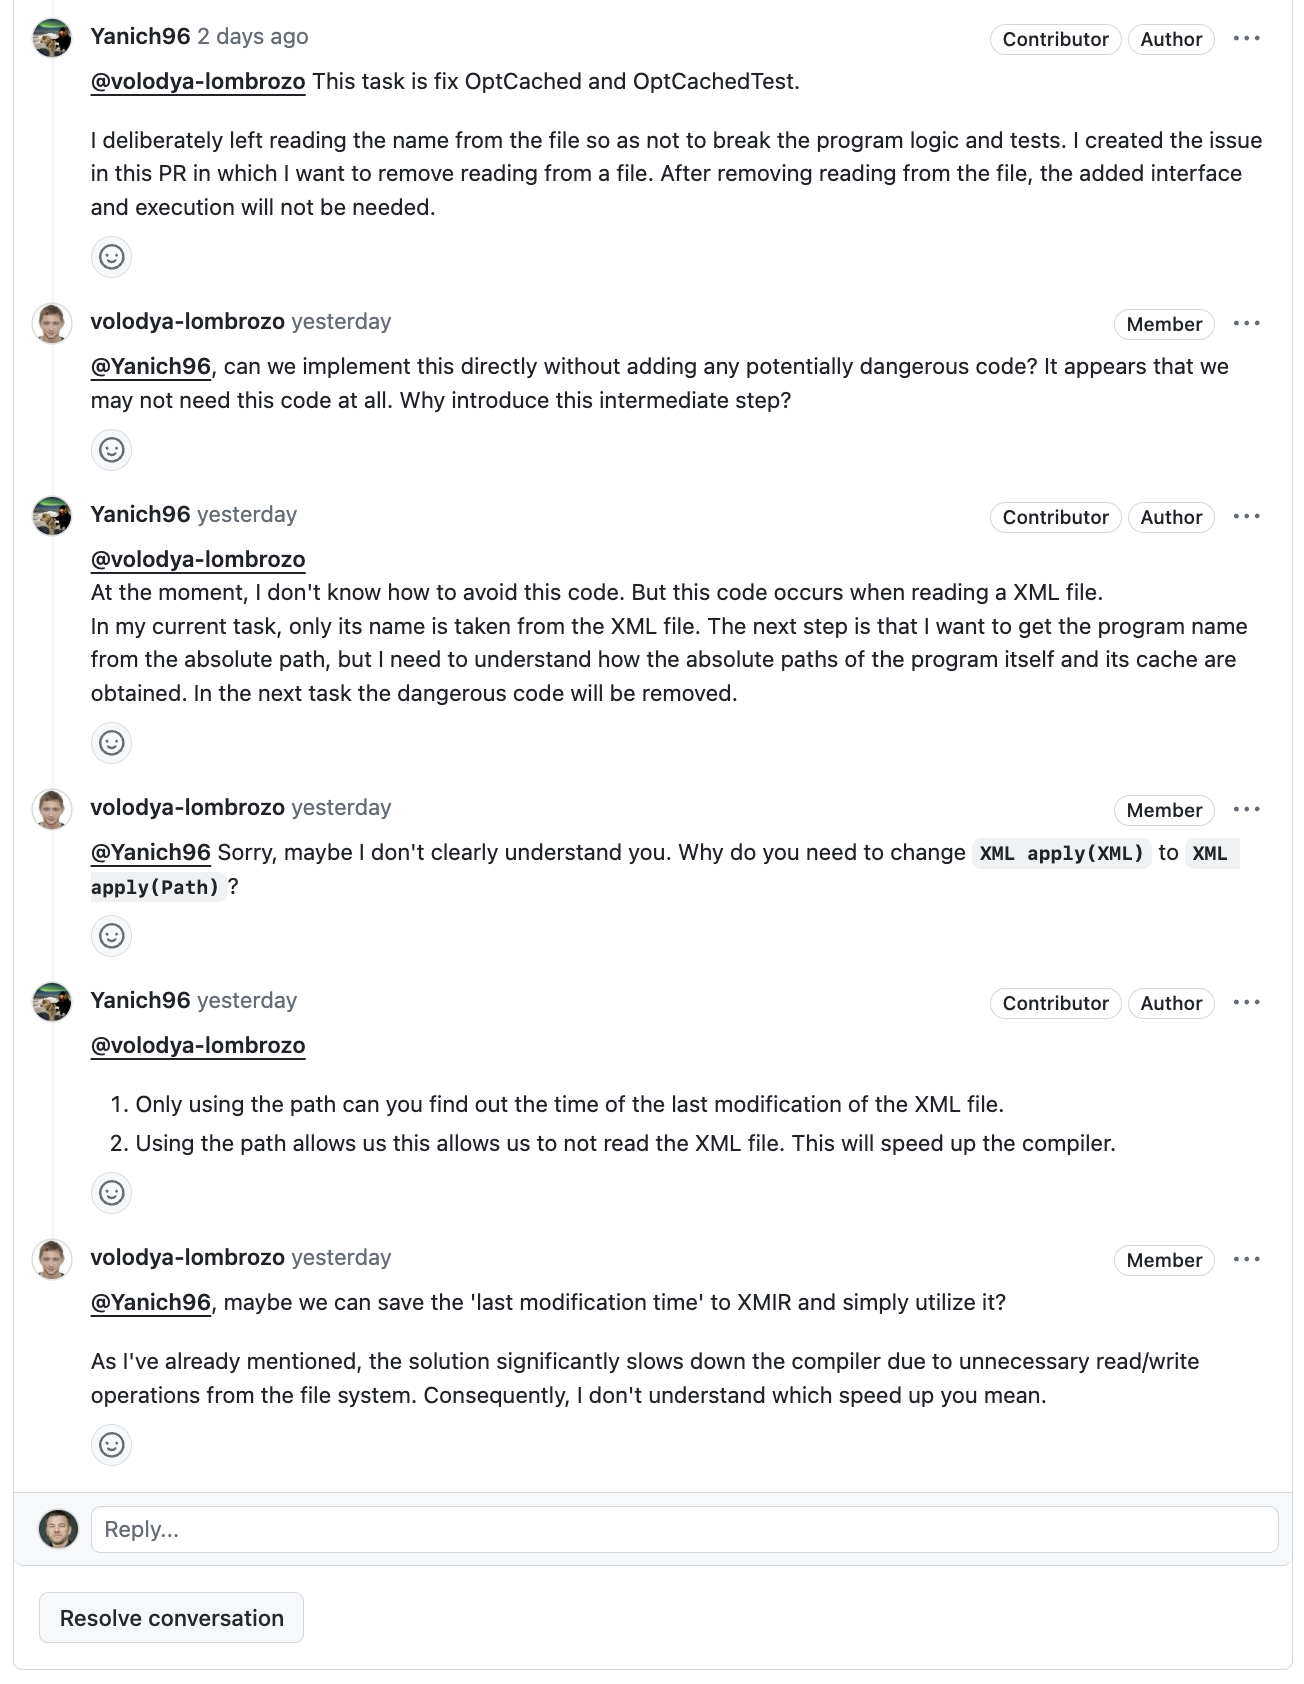
\includegraphics[width=.7\linewidth]{discussion.png}
  \par\columnbreak\par
  Every message starts with a nickname of the person
  who is the \ul{opponent} in the conversation.
  \par
  Github pull request:
  \href{https://github.com/objectionary/eo/pull/2808}{objectionary/eo\#2808}
  \end{multicols}
}

\thought{In an argument, provide \ul{links} that support your point of view.}

\thought{Beautify your profile, start with an anthropomorphic avatar.}

\qte
  [Kristine Nowak]
  {kristine-nowak}
  {Avatars that were more \ul{anthropomorphic} were perceived to be more \ul{attractive} and \ul{credible}. The strongest predictor of these variables, however, was the degree of masculinity or femininity (lack of androgyny) of an avatar.}
  {nowak2005influence}

\qte
  [Josh Terrell]
  {josh-terrell}
  {Surprisingly, our results show that women's contributions tend to be accepted \ul{more often} than men's. However, for contributors who are outsiders to a project and their gender is identifiable, men's acceptance rates are \ul{higher}.}
  {terrell2017gender}

\qte
  [Reza Nadri]
  {reza-nadri}
  {We have identified that submitters perceptible as Hispanic and Black have 39\% of their pull requests rejected because they are seen as unnecessary, which is 10-12 percentage points more frequent than the rest of perceptible races.}
  {nadri2021insights}

\qte
  [Nasif Imtiaz]
  {nasif-imtiaz}
  {We found that women did not provide more information on competence and were not generally measured at a stricter standard than men. We observed that women were less likely to express \ul{politeness} and \ul{profanity} than men, and were more restrictive in expressing their \ul{sentiments} on the platform.}
  {imtiaz2019investigating}

\qte
  [Carolyn D. Egelman]
  {carolyn-egelman}
  {Being a \ul{new employee} is not a statistically significant predictor of any of our feelings of pushback. Compared to authors at level 1 (entry level), authors at level 3 are 28\% less likely to see conflict in their code review changes.}
  {egelman2020predicting}

\pitch{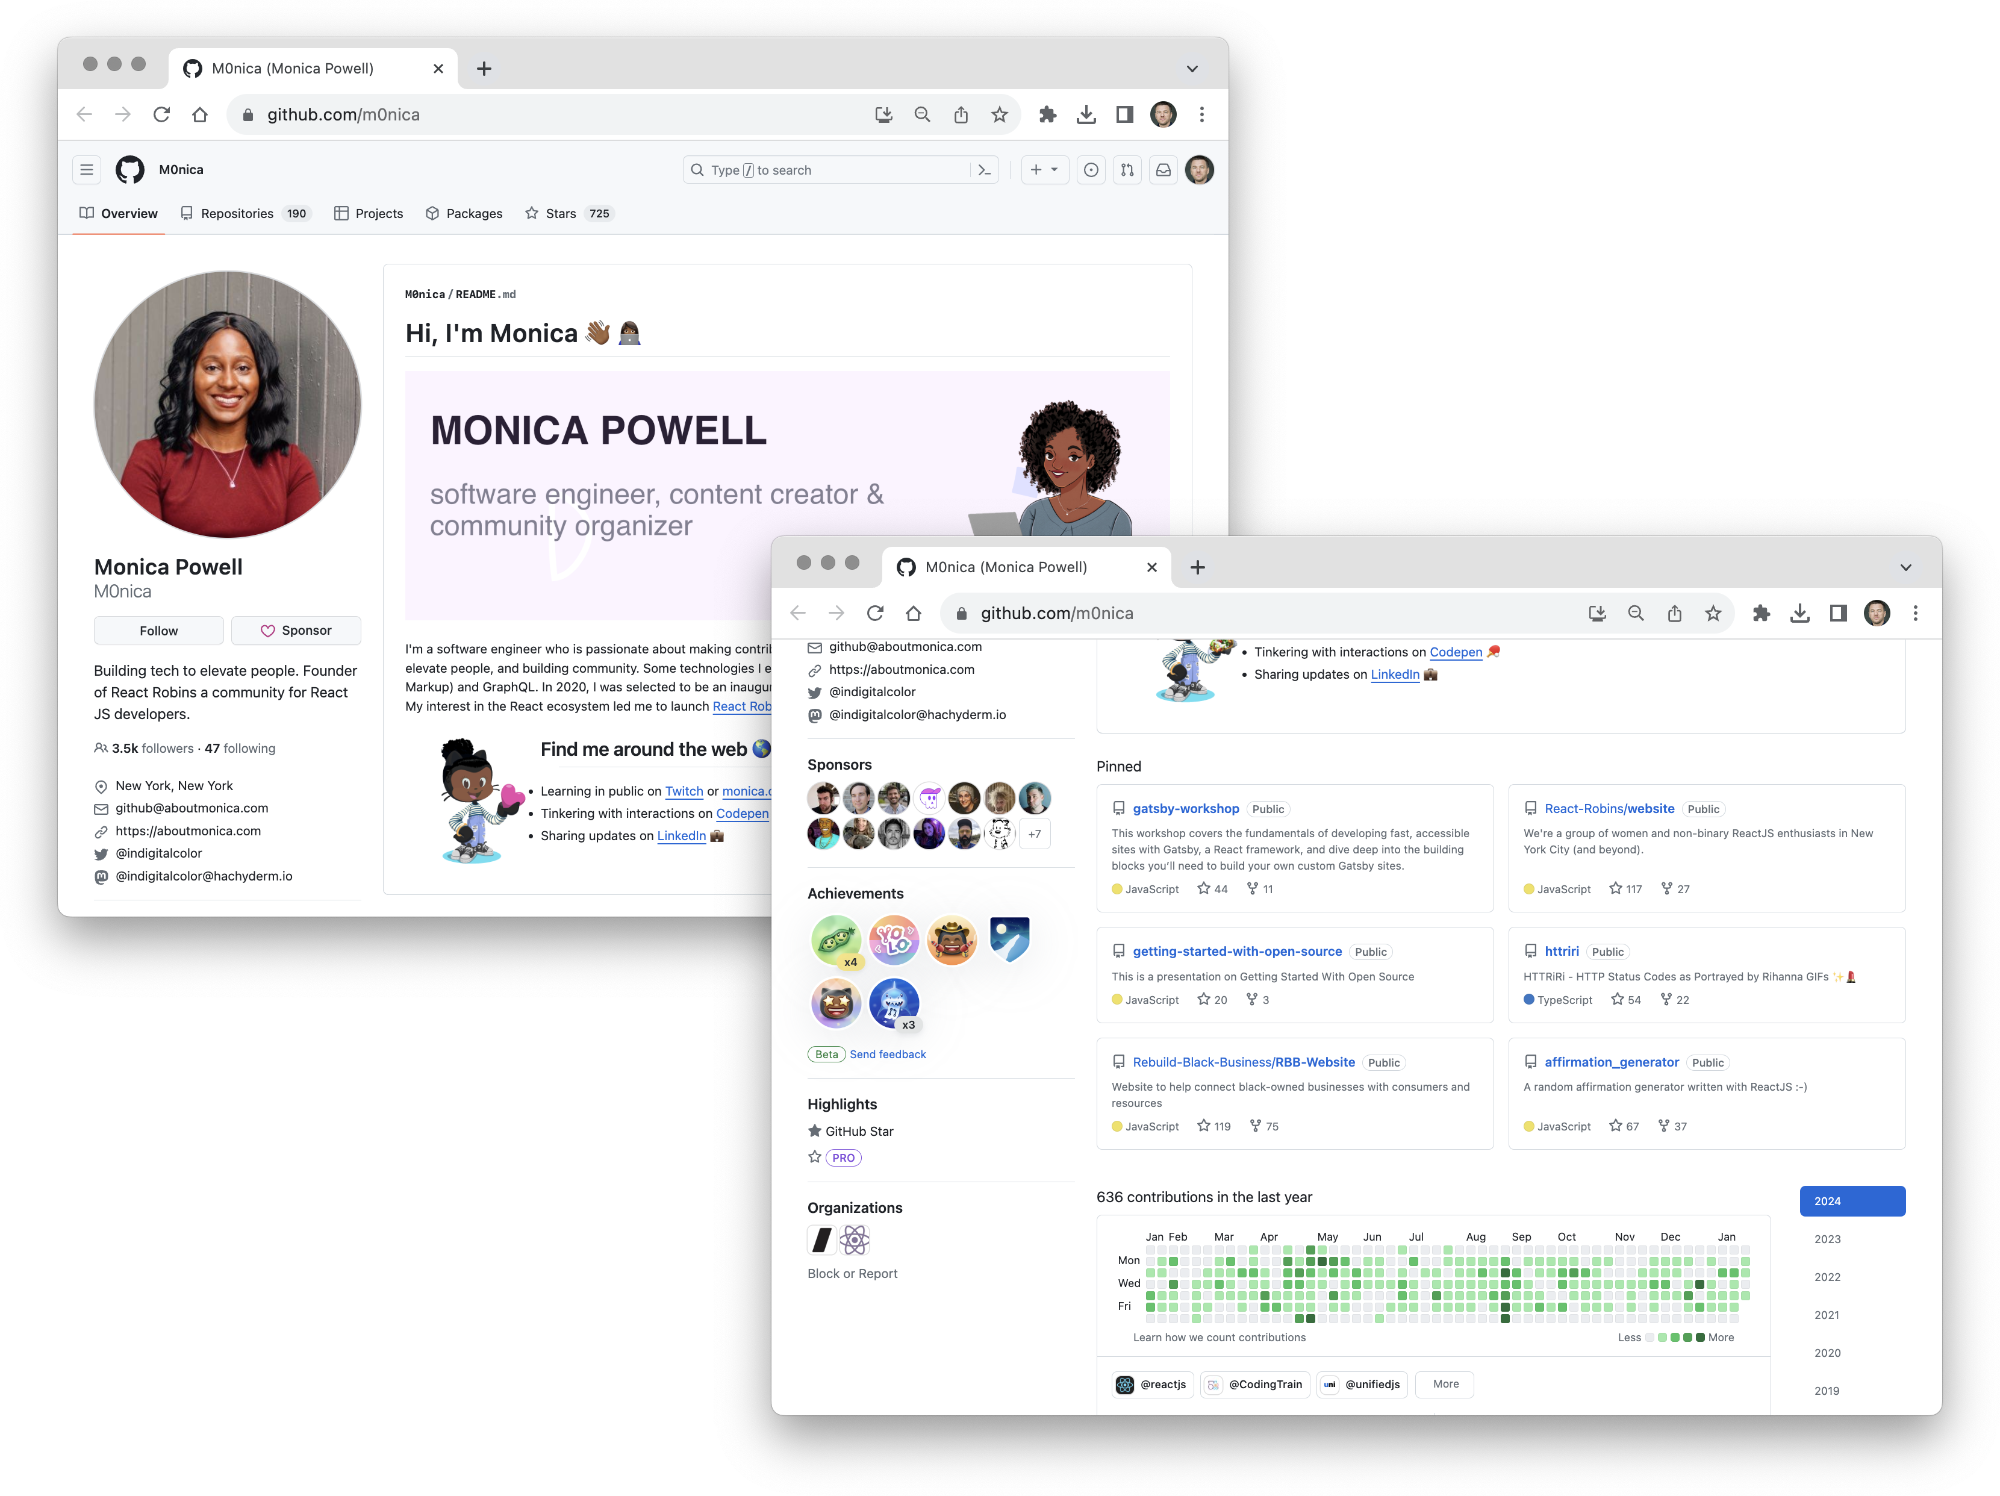
\includegraphics[width=.75\linewidth]{monica.png}}

\thought{Stay in the ticket, don't escape to Telegram, Slack, or an office debate.}

\qte
  {mark-warschauer}
  {The findings showed a tendency toward \ul{more equal} participation in computer mode. Students used language which is lexically and syntactically \ul{more formal} and complex in electronic discussion than they did in face-to-face discussion, thus demonstrating another possible advantage of computer-mediated communication.}
  {warschauer1995comparing}

\pitch{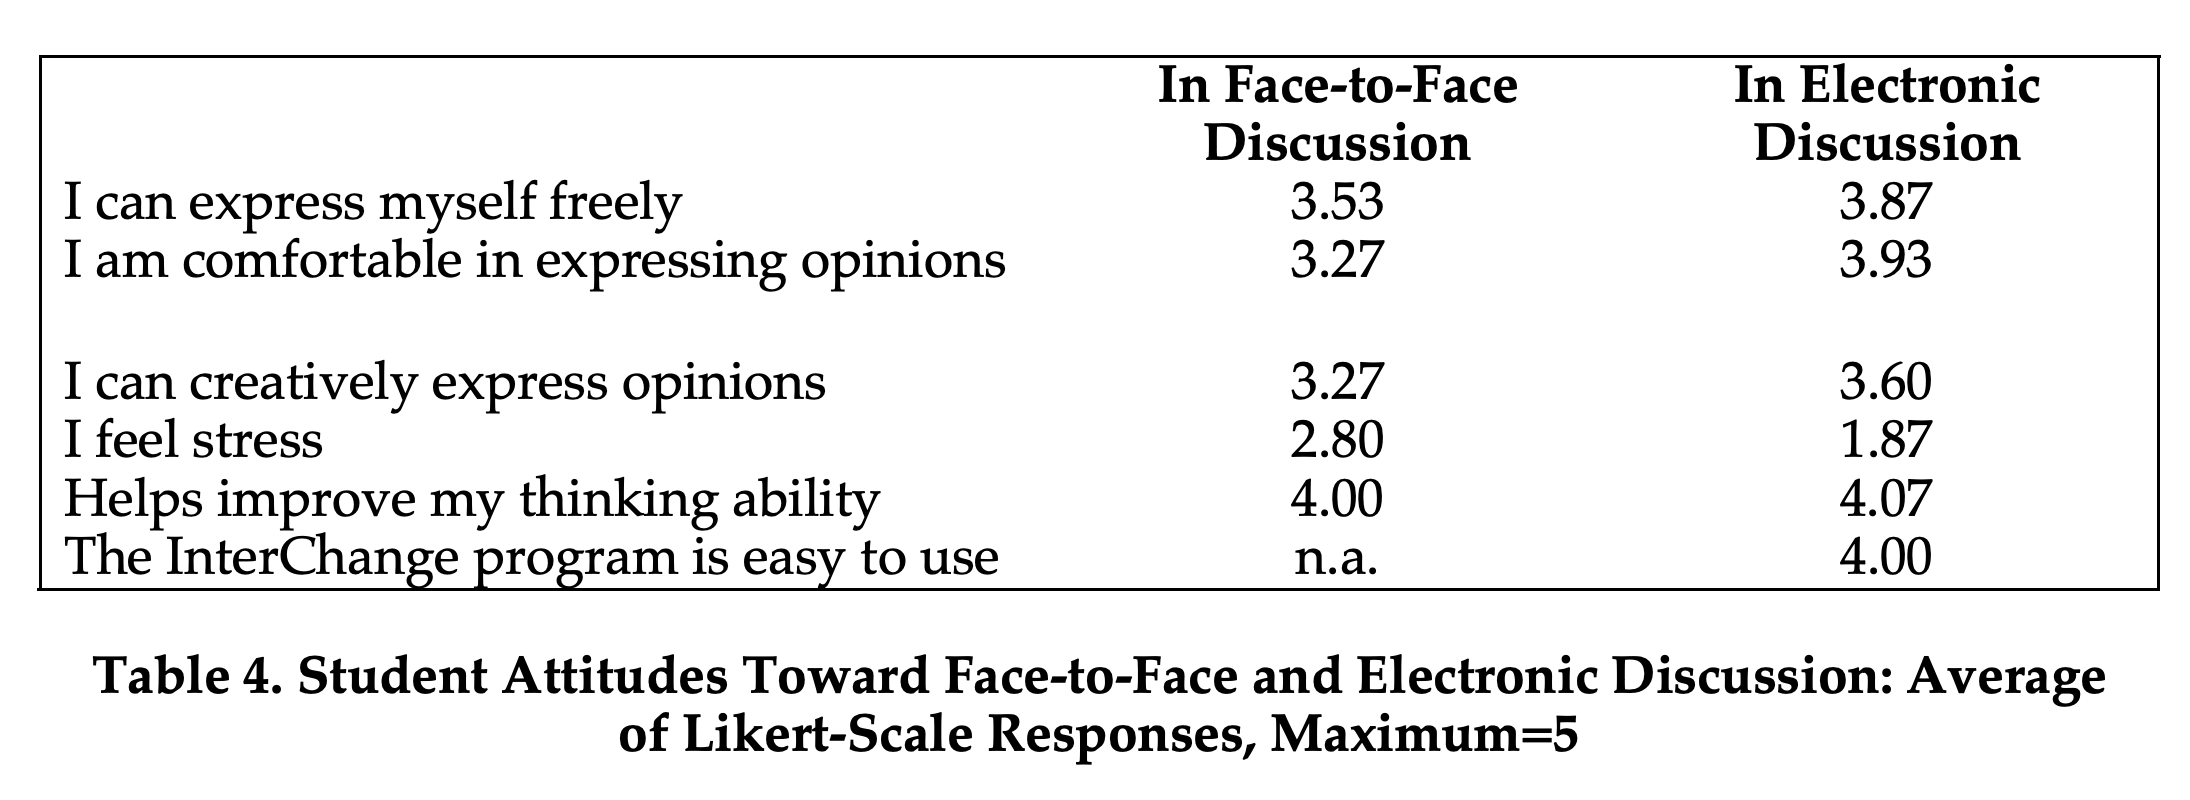
\includegraphics[width=\linewidth]{face-to-face.png}}

\qte
  [Verena Ebert]
  {verena-ebert}
  {Developers use many channels. Previously, mailing lists were very common. Nowadays, other communication channels become more and more popular, for example, Slack, issue trackers, Twitter or Gitter.}
  {ebert2022communication}

\pitch{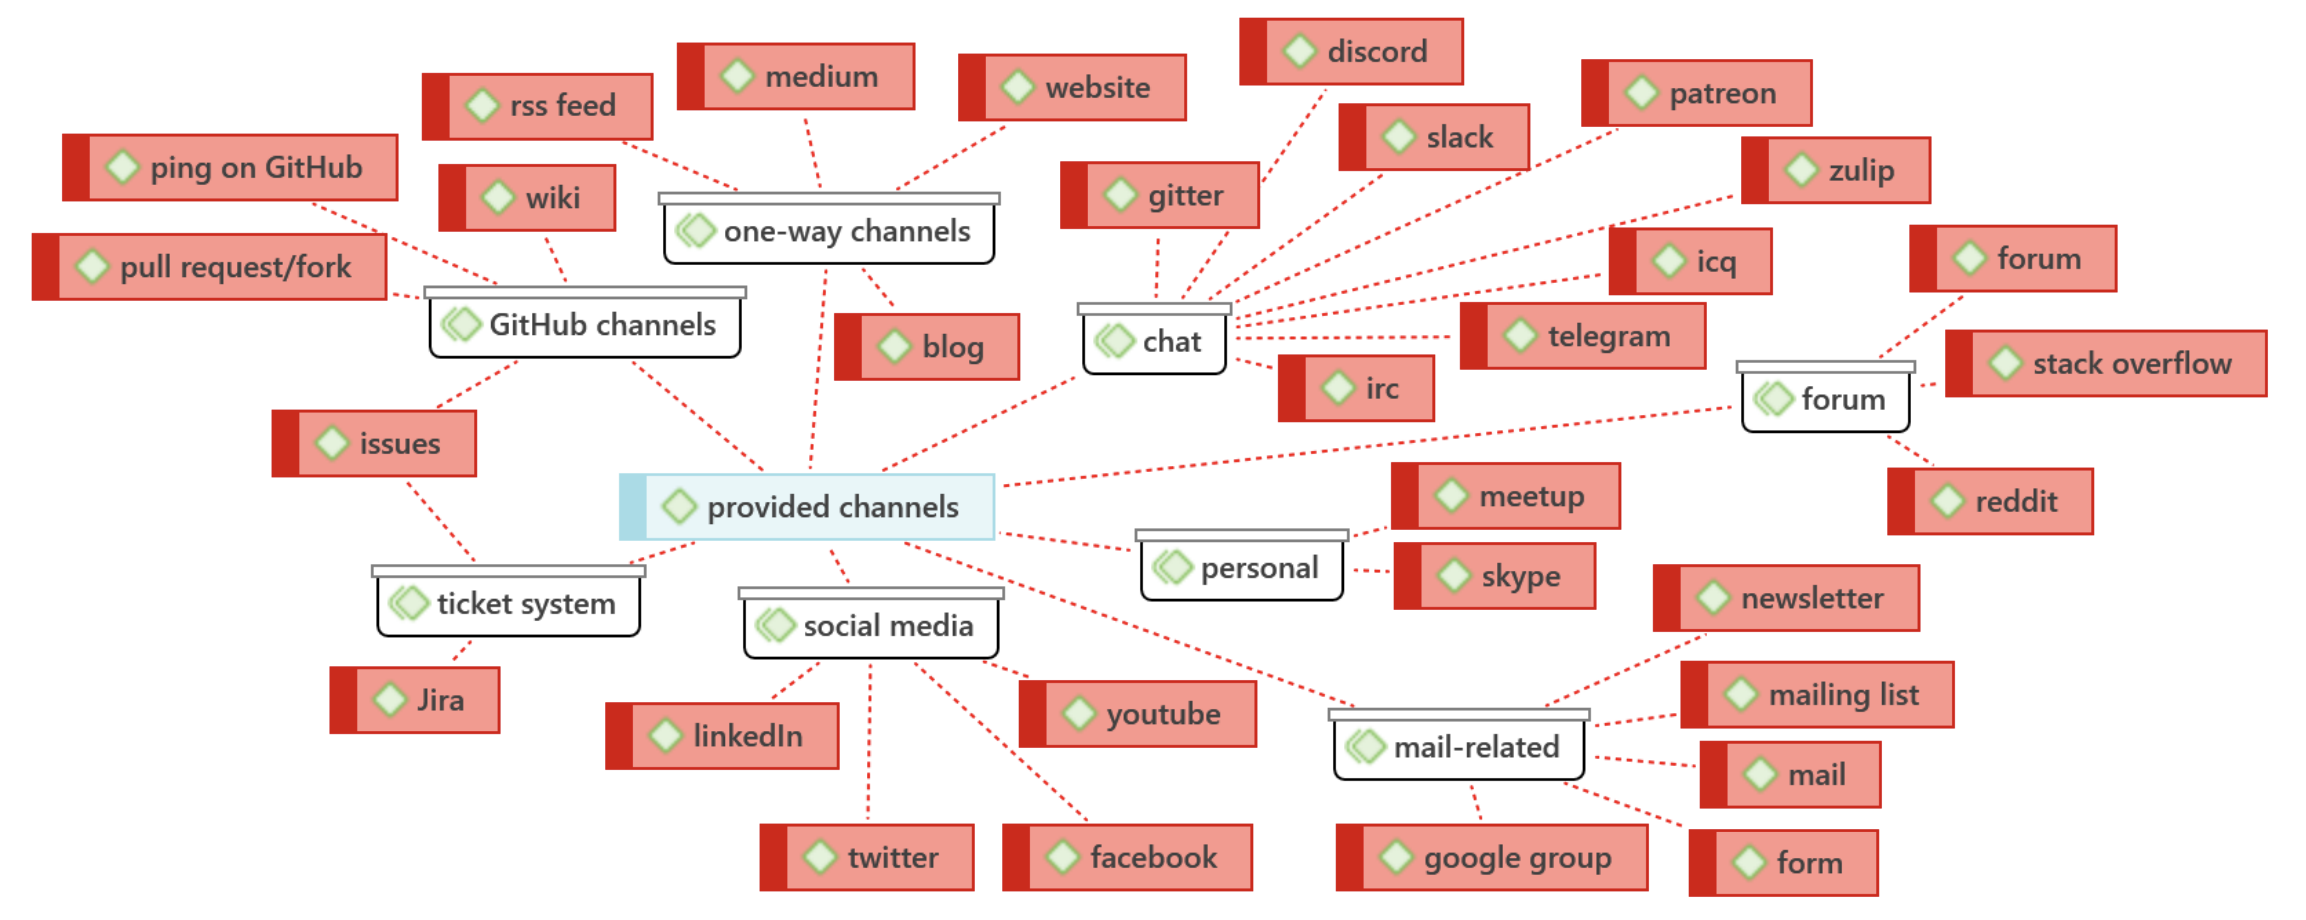
\includegraphics[width=.9\linewidth]{channels.png}}

\thought{Be polite, especially when you are angry or disagree.}

\qte
  [Xuan Lu]
  {xuan-lu}
  {Developers who use emojis in their posts are significantly less likely to dropout from the online work platform.}
  {lu2022emojis}

\qte
  [Thomas Fackler]
  {thomas-fackler}
  {Our results show that there is \ul{gravity} in online collaborations on GitHub. Traditional determinants of international trade such as \ul{language barriers} and \ul{country borders} matter for international code contributions.}
  {fackler2020gravity}

\qte
  {nadzeya-laurentsyeva}
  {The \ul{conflict} exerted a strong and persistent negative effect on the overall
  Ukrainian-Russian collaboration as measured by Ukrainian contributions
  to Russian projects and vice versa. The effect is \ul{symmetric} on the extensive margin.
  However, on the intensive margine, Ukrainian programmers react stronger: conditional
  on collaborating with Russians, they contribute to \ul{fewer} Russian projects.}
  {laurentsyeva2019friends}

\qte
  [Justin Middleton]
  {justin-middleton}
  {While we indeed find support for the idea that increases in activity correlate with a higher probability for membership, we also found the particular cases for which more activity can reduce the probability. This underscores the notion that software collaboration is much more than the code itself and that the social components of software should not be undervalued by software teams.}
  {middleton2018contributions}

\qte
  {pope-francis}
  {Pope Francis offered some Valentine’s Day advice Friday for a lasting marriage, telling 25,000 \ul{lovebirds} that the recipe for success lies in saying three simple words: `\ul{Please}, \ul{thanks} and \ul{sorry}.'{}}
  {pope2014}

\end{document}
